\subsection{Processo de Desenvolvimento: Nível de Programa e Time}

O gerenciamento da sprint foi feito por quadros Kanban, na qual teremos nove quadros principais. Esses quadros se encontram nos Boards do github, utilizando como base o plugin chamado \href{https://www.zenhub.com/}{Zenhub}. Para instalar é só baixar o plugin e instalar no navegador, a partir daí já conseguirá ver toda organização das issues do projeto a partir da ferramenta. Os quadros são:

\begin{itemize}
  \item \textbf{Epic}: Épicos do software.
  \item \textbf{Features}: \textit{Features} do software.
  \item \textbf{New issues}: Novas histórias de usuário, bug reports ou qualquer tipo de situações de trabalho relacionadas ao desenvolvimento da aplicação que ainda não foram mapeadas, pontuadas ou priorizadas e consequentemente alocadas nos demais quadros.
  \item \textbf{Ice Box}: Issues congeladas por dependência de outras, por alguma necessidade de reavaliação da necessidade ou do esforço necessário para concluí-la, por dependência de funcionalidades externas que não são disponibilizadas pelos mantenedores, por temporária incapacidade da equipe de solucionar determinado problema, etc.
  \item \textbf{Product Backlog}: \textit{Board} para histórias/tarefas ou correções já mapeadas e priorizadas. É importante esclarecer que nesse quadro, a prioridade é definida pela posição da \textit{issue} na \textit{board}, sendo que as posições superiores determinam maior relevância para o projeto.
  \item \textbf{Sprint Backlog}: \textit{Issues} alocadas para os pares na \textit{sprint} corrente ou \textit{bug fixes} de alta prioridade.
  \item \textbf{Review}: Tarefas concluídas que necessitam de revisão para entrarem na aplicação.
  \item \textbf{Done}: Código já revisado que pode ser anexado a aplicação na próxima release.
  \item \textbf{Closed}: \textit{Issues} fechadas já anexado a aplicação.
\end{itemize}

Na figura \ref{fig:desenvolvimento} está definido o processo de desenvolvimento que está no nível de programa e time.

\begin{figure}[h!]
	\centering
  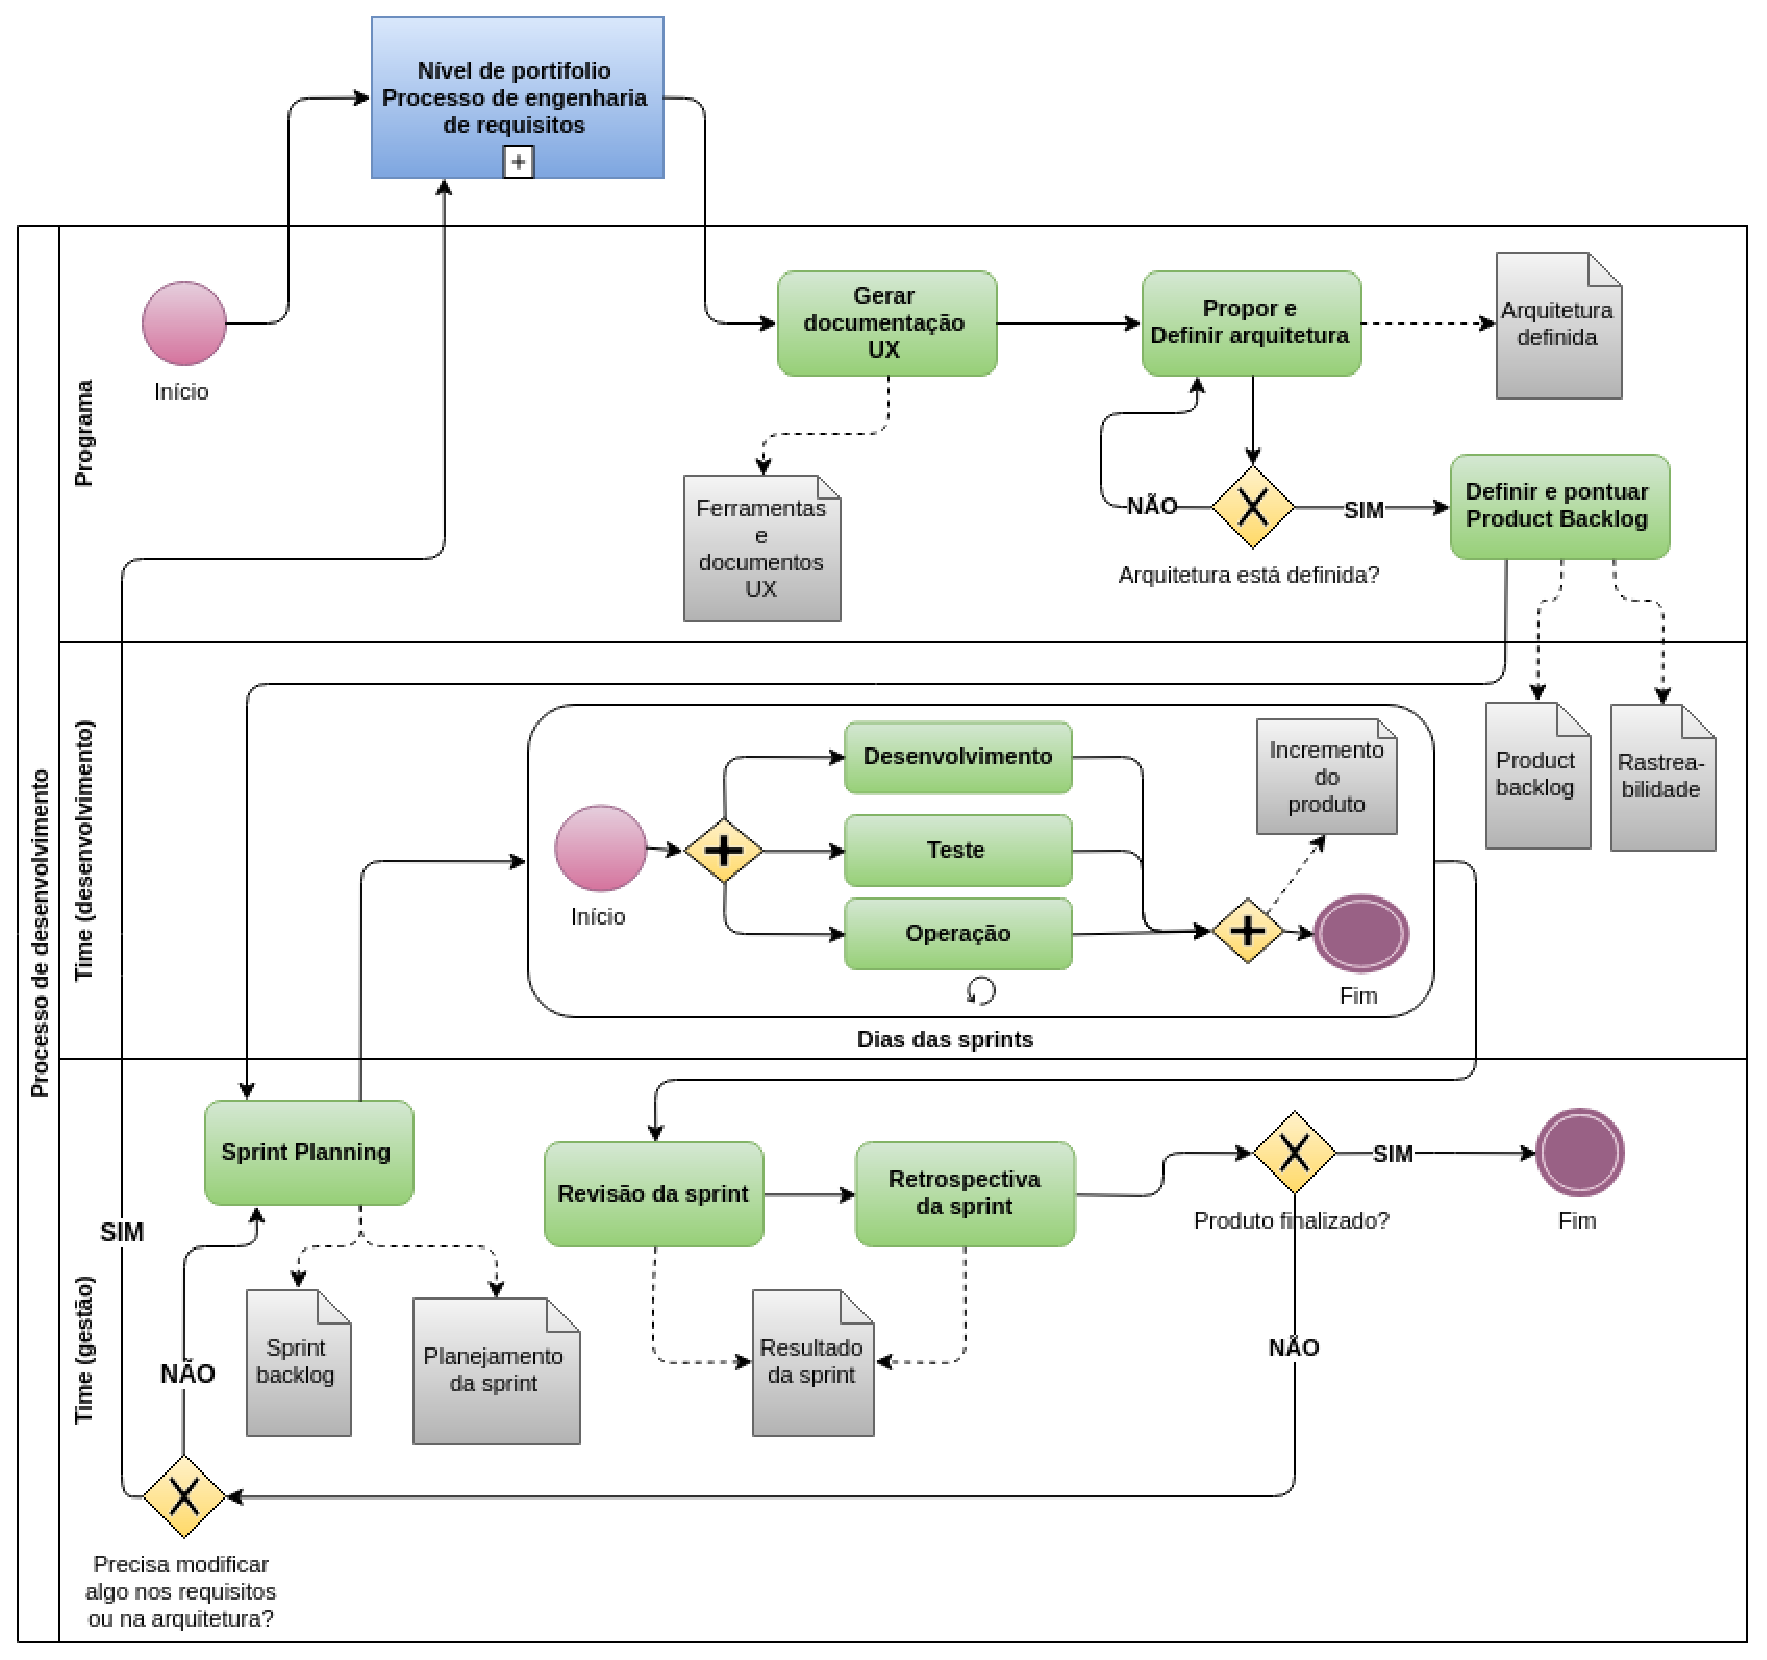
\includegraphics[keepaspectratio=true,scale=0.5]{figuras/desenvolvimento.eps}
  \caption[Processo de desenvolvimento.]{Processo de desenvolvimento. Fonte: Autor}
	\label{fig:desenvolvimento}
\end{figure}

Todo processo definido será executado de forma incremental por iterações, ou seja, a cada iteração será realizada um
refinamento dos documentos e um incremento do produto, essas iterações são chamadas \textit{Sprints}.

\subsubsection{Nível de Programa}

Fase responsável pela auto-organização de times ágeis, entrega contínua de valor, criação de Features por meio dos épicos encontrados, realização de toda a documentação relacionada ao \textit{User Experience} ou UX, e definição do documento de arquitetura do software.

\begin{itemize}
  \item \textbf{Gerar documentação UX}:
  \begin{itemize}
    \item \textbf{Descrição}: Nesta etapa, objetiva-se criar os documentos UX relevantes para o projeto como
      protótipos, sitemaps, entre outros.
    \item \textbf{Entradas}: Requisitos e modelos
    \item \textbf{Saídas}: Ferramentas e documentos UX como sitemap, StoryBoards e Prototipo
  \end{itemize}
  \newpage
  \item \textbf{Propor e definir arquitetura}:
  \begin{itemize}
    \item \textbf{Descrição}: Nesta etapa, objetiva-se propor e definir a arquitetura que melhor se adapte ao projeto
      e a equipe.
    \item \textbf{Entradas}: Requisitos e modelos
    \item \textbf{Saídas}: Documento de arquitetura
  \end{itemize}
  \item \textbf{Definir e pontuar product backlog}:
  \begin{itemize}
    \item \textbf{Descrição}: Nesta etapa, objetiva-se definir e pontuar as histórias de usuário do product backlog
      para a release que segue.
    \item \textbf{Entradas}: Features e Enables
    \item \textbf{Saídas}: Product Backlog e Rastreabilidade.
  \end{itemize}
\end{itemize}

\subsubsection{Nível de Time}

Fase responsável pelo auto-gerenciamento da equipe ágil, incremento do software totalmente testado, práticas SCRUM e XP, descrição do valor por meio de User Stories e tarefas.

\begin{itemize}
  \item \textbf{Sprint Planning}:
  \begin{itemize}
    \item \textbf{Descrição}: Nesta etapa, objetiva-se priorizar as histórias de usuários que serão implementadas na
      iteração/sprint que se segue. Os planejamentos e Resultados encontram-se na wiki do projeto.
    \item \textbf{Entradas}: Product Backlog
    \item \textbf{Saídas}: Sprint Backlog e Planejamento das sprints
  \end{itemize}
  \item \textbf{Ciclo de dias das sprints}:
  \begin{itemize}
    \item \textbf{Descrição}: Nesta etapa, será aplicado às boas práticas do SCRUM e XP em nível de desenvolvimento.
      Foram retirados algumas atividades do SCRUM como Daily Scrum, e práticas XP como programação pareada, já que
      a equipe é composta de um único membro, não há como fazer. Dentro dessa atividade temos em paralelo o
      desenvolvimento, teste e operações do incremento do produto.
    \item \textbf{Entradas}: Sprint Backlog
    \item \textbf{Saídas}: Incremento do produto testado e em homologação
  \end{itemize}
  \item \textbf{Revisão da sprint}:
  \begin{itemize}
    \item \textbf{Descrição}: Nesta etapa, será apresentado as funcionalidades implementadas na sprint e verificar
      se há alguma dívida técnica para a próxima sprint que se segue, aqui entra o processo de verificação e validação.
    \item \textbf{Entradas}: Incremento do produto
    \item \textbf{Saídas}: Resultados da sprint
  \end{itemize}
  \item \textbf{Retrospectiva da sprint}:
  \begin{itemize}
    \item \textbf{Descrição}: Nesta etapa, será coletado pontos positivos, negativos e melhorias para as próximas
      iterações da equipe
    \item \textbf{Entradas}: Pontos positivos, negativos e melhorias
    \item \textbf{Saídas}: Resultados da sprint
  \end{itemize}
\end{itemize}

